% NOMAD Design Overview. Dr. Lin's text from lin_draft/main_20261019.tex (lines 150-188, 197-201)
% is installed word for word; only empty or placeholder cross-references are filled. His [Archive]
% paragraph "The Framework's Objective" with R01-R03 (lines 190-195) is replaced by the objectives
% paragraph below, which the Evaluation answers one to one.
\section{NOMAD Design Overview}
\label{sec:overview}
In this section, we first present the threat model used by current ICS device fingerprinting. The assumptions about adversaries lead to NOMAD's design principles and major building components. 
%We describe the adversary, their capability, and their knowledge, and then go into our research objectives, which the framework must achieve.
\subsection{Threat Model}

\begin{figure}[t]
\centering
\IfFileExists{figures/fig_observation.pdf}{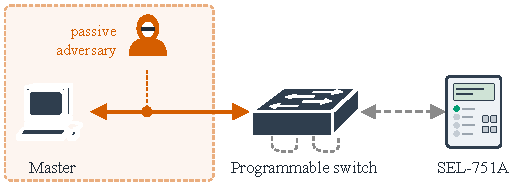
\includegraphics{figures/fig_observation}}{\figplaceholder{Observation model: master, observed master-facing link, programmable switch, relay-facing link (not observed), SEL-751A outstation.}}
\caption{Observation model. The adversary monitors the shaded master-facing link. The dashed paths
  are not visible to it.}
\label{fig:observation}
\end{figure}

\textbf{Assumptions on Adversary's Capability.} We  assume the adversary has penetrated the control network already and can passively monitor traffic from the  master-facing link as shown in Figure~\ref{fig:observation}. The passive observer is able to read and record packet headers, their sizes, and arrival time, and because DNP3 does not have any transport security by default~\cite{east2009}, this gives the observer the ability to read the function codes of each request, and using that, they are able to label each exchange by what it does, e.g., READ poll or SELECT and OPERATE. We also assume that the adversary knows the existence of the framework and the intervals it obfuscates, but they cannot read the internal mechanism and state of the switch or be able to monitor the link between the switch and the outstation. This is practical, as the switch usually sits at  the edge of the outstation and is usually connected with a single cable between devices in the same substation cabinet.

\textbf{Adversary's Goal.} The aim of the adversary is to fingerprint the outstation using the timing from the exchanges and then infer the make and model of devices and the operation each of them performs. With this knowledge, they can design specific and targeted attacks like false data injection that must match the devices they compromise~\cite{liufdia2009}.
We consider an  adversary that builds its classifier from captured traffic before the framework is deployed and applies it afterwards.

\subsection{Design Goals}

Before describing NOMAD's design goal, we use a sample network trace collected from IEDs from two different vendors, i.e., the Schweitzer Engineering Laboratories (SEL) 751A~\cite{sel751a} and the Schneider Electric (SE) ION7550 power meter~\cite{seion7550}, to demonstrate unique characteristics in ICS device fingerprinting. First, despite establishing security extensions in common ICS network protocols, plain-text communication is still prevalent in power grids and other ICSs. We have developed a web crawler that examined public product manuals, datasheets, and pages from five IED vendors, namely, SEL, SE, Rockwell Automation, GE Vernova, and Siemens. With a stratified sample of 99 catalogued entries, 32 were identified as having DNP3 support, and these documents established encryption for six entries, and one had DNP3 authentication. However, it is also established that OT asset owners and operators do not use these security measures even if they exist, with numerous reasons hindering their adoption~\cite{CISA2026SecureOT}. The crawler methodology and detailed results are presented in Appendix~\ref{app:crawler}.

% TODO web crawler on SEL, SE, AB, GE, Siemens product to see their support of security functionality.  

Second, different IEDs can configure network protocols differently, and some even include undocumented variants. These configurations, largely benefiting from plain-text communication, can enable ad hoc features for ICS device fingerprinting. In Figure~\ref{fig:motivation}, we present the data acquisition based on the DNP3 protocol on IEDs from two different vendors, i.e., the Schweitzer Engineering Laboratories (SEL) 751A~\cite{sel751a} and the Schneider Electric (SE) ION7550 power meter~\cite{seion7550}. Based on the network trace, we find that SEL 751A disables TCP's ``delayed ACK'' mechanism, making CLRT a viable fingerprinting feature. However, SE ION7550 enables this mechanism, so we can no longer use CLRT to estimate how long the device spent retrieving measurements.  and configure the DNP3 protocol with different parameters. We believe the proprietary network protocol implementation and configuration can form unique device fingerprints, which also present an excellent opportunity to disrupt adversaries' reconnaissance if a different device fingerprint can be manipulated.

\begin{figure}[t]
\centering
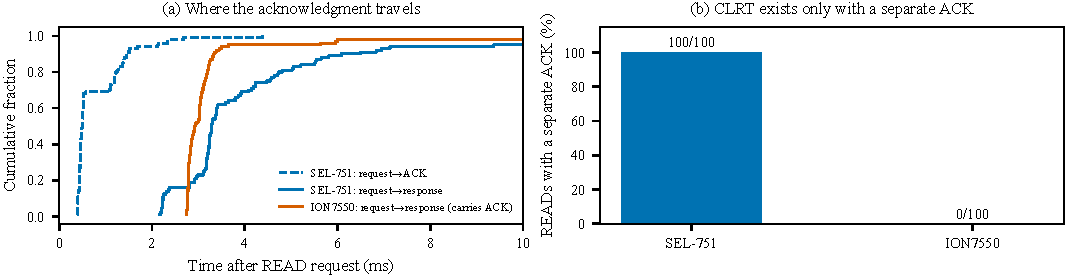
\includegraphics[width=\columnwidth]{figures/nomad_eval/fig_motivation}
\caption{The same Class~0 READ poll on two IEDs behind the testbed switch. (a) The SEL-751A acknowledges each request in a separate TCP segment, so its CLRT exists; the ION7550 lets the response carry the acknowledgment. (b) Share of READ polls with a separate acknowledgment, 100 polls per device.}
\label{fig:motivation}
\end{figure}

To counter unique ICS device fingerprinting, we design NOMAD driven by the following goals.  

\begin{itemize}[leftmargin=*,labelindent=0pt,labelsep=12pt, listparindent= 12pt,topsep=0pt, itemsep=0pt, parsep=0pt]

\item \textbf{Obfuscation over Plain-text.} Despite ICS network protocols are gradually enhanced with security components, plain-text communication still prevails in ICS due to existing legacy devices and demanding communication requirements. It is essential to apply various obfuscation strategies, including packet splitting and padding, over plain-text communication without revealing the fact. 

\item \textbf{Flexible Obfuscation.} Features from different types of network packets can combine to form unique fingerprints for IEDs. Applying different obfuscation strategies based on packet types and extracted features is important to accommodate ad-hoc fingerprinting methods.

\item \textbf{Low Runtime Overhead.} Maintaining constant latency while applying various obfuscation strategies on thousands of IEDs in a power grid is essential to disrupt diverse device fingerprinting. 

\item \textbf{No Reliance on De-obfuscation.} If we follow existing obfuscation solutions, a de-obfuscation unit processes network traffic from obfuscated traffic from all IED, presenting security and overhead bottleneck. It is critical to make obfuscation directly protocol-conformance, putting no reliance on de-obfuscation.  

\end{itemize}

\textbf{Objectives.} To make these goals concrete for the transactions in Fig.~\ref{fig:ladder}, NOMAD pursues three research objectives, which the evaluation answers one by one (Section~\ref{sec:evaluation}).
\begin{itemize}[leftmargin=*,labelindent=0pt,topsep=2pt,itemsep=1pt,parsep=0pt]
\item \textbf{RO1:} For READ, SELECT and OPERATE, the timing a passive observer measures on the master-facing link equals values that the operator configures, independent of how fast the outstation serves the request.
\item \textbf{RO2:} Every response carries the same number of bytes and the same control units, and remains conformant to IEEE~1815, so that neither the master nor the outstation needs a de-obfuscation unit.
\item \textbf{RO3:} The added delay stays within the DNP3 and TCP timers of the master, so that no request is retransmitted, and the whole mechanism fits one programmable switch.
\end{itemize}

\textbf{Trusted Components.} To make these objectives possible, we only add a switch and a control plane to the trusted computing base. The control plane installs the policy to the switch for enforcement. The master or the outstation is not needed, and neither are they modified for the framework to function.

\subsection{Components and Workflows}

As shown in Fig.~\ref{fig:components}, NOMAD includes two components: (i) \textit{Obfuscation infrastructure} that uses P4-enabled network data planes to apply flexible obfuscation strategies and (ii) \textit{obfuscation objectives/constraints} determining security properties in various scenarios while observing ICS communication requirements. When a network packet traverses a gateway network device, we use a customized parser to extract network attributes and control-related knowledge, then categorize packets and organize the carried control units accordingly in the switch's local storage. Using the control-unit syntax, including sizes and indices, we can split, pad, and schedule control units according to different operations while maintaining protocol compliance. While obfuscation infrastructures provide an in-network hardware foundation, we use switches' control plane to realize various obfuscation objectives under constraints for diverse security applications, e.g., neutralize, mimicry communication patterns, and/or maximize differences between obfuscated and original patterns.  

\begin{figure*}[t]
\centering
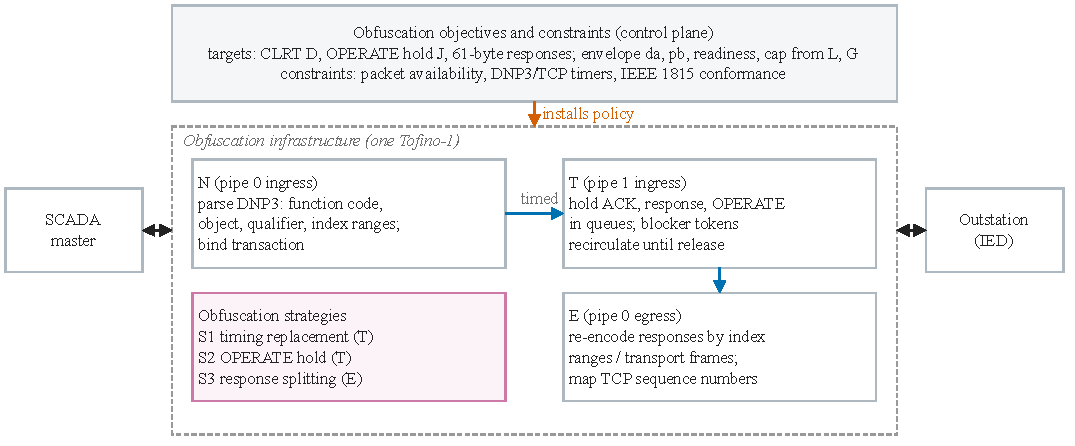
\includegraphics[width=\textwidth]{figures/nomad/fig_nomad_components}
\caption{NOMAD's components. The control plane installs the obfuscation objectives and constraints. On one Tofino-1 switch, program N parses DNP3 and binds each transaction, program T holds acknowledgments, responses and OPERATE commands in queues while blocker tokens recirculate, and program E re-encodes responses and maps TCP sequence numbers.}
\label{fig:components}
\end{figure*}
